
\documentclass[hyperref={pdfpagelabels=false},ngerman]{beamer}

% stop font warning
\let\Tiny=\tiny
\providecommand\thispdfpagelabel[1]{}

\usepackage[english]{babel}
\usepackage{lmodern}
\usepackage[T1]{fontenc}
\usepackage[utf8]{inputenc}
\usepackage{graphicx,import}
\usepackage{feynmp}
\DeclareGraphicsRule{*}{mps}{*}{} 
\DeclareGraphicsExtensions{.pdf}
\usepackage{amsmath,amssymb,amstext,amsfonts} % mathrsfs
\usepackage{array,booktabs,tabularx}
\usepackage{tikz,tikz-uml,pgf-pie}
\usetikzlibrary{shapes,calc,arrows,positioning}
\tikzstyle{block} = [rectangle, draw, text width=7em, text centered, minimum height=2em]
\tikzstyle{arrow} = [draw, -latex, thick]
\tikzstyle{arrow2} = [draw, latex-latex, thick]
\tikzstyle{quark}  = [rectangle, draw, fill=yellow, minimum width=2em, text centered, minimum height=2em]
\tikzstyle{lepton} = [rectangle, draw, fill=red!50, minimum width=2em, text centered, minimum height=2em]
\tikzstyle{gauge}  = [circle   , draw, fill=green , minimum size=2em, inner sep=0pt, text centered]
\tikzstyle{scalar} = [diamond  , draw, fill=blue!40, minimum width=2.3em, text centered, minimum height=2.3em, inner sep=0pt]
\tikzstyle{goldstone} = [diamond, draw, dashed, fill=blue!30, minimum width=2.3em, text centered, minimum height=2.3em, inner sep=0pt]
\tikzstyle{squark}   = [diamond, draw, fill=yellow, minimum width=2.3em, text centered, minimum height=2.3em, inner sep=0pt]
\tikzstyle{slepton}  = [diamond, draw, fill=red!50, minimum width=2.3em, text centered, minimum height=2.3em, inner sep=0pt]
\tikzstyle{gaugino}  = [rectangle, draw, fill=green , minimum size=2em, inner sep=0pt, text centered]
\tikzstyle{higgsino} = [rectangle, draw, fill=blue!40  , minimum width=2em, text centered, minimum height=2em]
\tikzstyle{inert}    = [diamond  , draw, fill=teal!80, minimum width=2.3em, text centered, minimum height=2.3em, inner sep=0pt]
\tikzstyle{inertino} = [rectangle, draw, fill=teal!80, minimum width=2em, text centered, minimum height=2em]
\tikzstyle{phantom}  = [rectangle, minimum width=2em, text centered, minimum height=2em]
\usepackage{slashed}
\usepackage{fixltx2e} % textsubscript
\usepackage{multirow}
\usepackage{tcolorbox}
\usepackage{pifont}
\usepackage{xspace}
\usepackage{hyperref}
\hypersetup{colorlinks,linkcolor=,urlcolor=blue}
\usepackage{listings}
\lstset{breaklines=true,
  breakatwhitespace=true,
%  numbers=left,
  numberstyle=\tiny,
  stepnumber=1,
  basicstyle=\ttfamily\footnotesize,
  commentstyle=\ttfamily\color{gray},
  postbreak={\mbox{{$\hookrightarrow$}}\space\space},
  breakindent=10pt,
  breakautoindent=false,
  showspaces=false,
  showstringspaces=false,
  frame=single}

\definecolor{darkgreen}{RGB}{0,176,0}

\newcommand{\cmark}{\ding{51}}%
\newcommand{\xmark}{\ding{55}}%
\newcommand{\fmfvcenter}[1]{\;\vcenter{\hbox{\fmfreuse{#1}}}\;}
\newcommand{\eh}[1]{\,\mathsf{#1}}
\newcommand{\ok}{\textcolor{darkgreen}{\cmark}}
\newcommand{\notok}{\textcolor{red}{\xmark}}
\newcommand{\maybe}{\textcolor{gray}{\cmark}}
\newcommand{\meh}{\textcolor{gray}{\textbf{\huge\lower.1em\hbox{-}}}}
\newcommand{\Lagr}{\mathcal{L}}
\newcommand{\MS}{\ensuremath{M_S}}
\newcommand{\mathi}{\mathsf{i}}
\newcommand{\mycite}[1]{\ensuremath{\text{\textcolor{darkgray}{\tiny [#1]}}}}
\newcommand{\bigcite}[1]{\textcolor{darkgray}{[#1]}}
\newcommand{\dimrep}[1]{\mathbf{#1}}
\newcommand{\dimrepadj}[1]{\mathbf{\overline{#1}}}
\newcommand{\ESSM}{E\textsubscript{6}SSM}
\newcommand{\CESSM}{CE\textsubscript{6}SSM}
\DeclareMathOperator{\tildeRe}{\widetilde Re}
\DeclareMathOperator{\sign}{sign}
\DeclareMathOperator{\re}{Re}
\DeclareMathOperator{\im}{Im}
\renewcommand{\emph}{\textbf}
\newcommand{\dd}{\mathsf{d}}
\newcommand{\myurl}[1]{\href{#1}{#1}}
\newcommand{\Superpot}{\mathcal{W}}
\newcommand{\SuperField}[1]{#1}
\newcommand{\ConjSuperField}[1]{\bar{#1}}
\newcommand{\UY}{\ensuremath{U(1)_{Y}}}
\newcommand{\UN}{\ensuremath{U(1)_{N}}}
\newcommand{\Uem}{\ensuremath{U(1)_\text{em}}}
\newcommand{\SUL}{\ensuremath{SU(2)_\text{L}}}
\newcommand{\SUc}{\ensuremath{SU(3)_\text{c}}}
\newcommand{\SOten}{\ensuremath{{SO(10)}}}
\newcommand{\comma}{,}
\newcommand{\DRbar}{\ensuremath{\overline{\text{DR}}}}
\newcommand{\MSbar}{\ensuremath{\overline{\text{MS}}}}
\newcommand{\SM}{\ensuremath{\text{SM}}}
\newcommand{\MSSM}{\ensuremath{\text{MSSM}}}
\newcommand{\pole}{\ensuremath{\text{pole}}}
\newcommand{\match}{\ensuremath{\text{match}}}
\newcommand{\tree}{\ensuremath{\text{tree}}}
\newcommand{\fsstar}{\textbf{*}}
\newcommand{\fs}{\texttt{FlexibleSUSY}\xspace}
\newcommand{\fsh}{\texttt{FS+H}\xspace}
\newcommand{\feft}{\texttt{FlexibleEFTHiggs}\xspace}
\newcommand{\hssusy}{\texttt{HSSUSY}\xspace}
\newcommand{\Himalaya}{\texttt{Himalaya}\xspace}
\newcommand{\FH}{\texttt{FeynHiggs}\xspace}
\newcommand{\SPheno}{\texttt{SPheno}\xspace}
\newcommand{\SARAH}{\texttt{SARAH}\xspace}
\newcommand{\Zv}{\ensuremath{\backslash\mkern-11.0mu{Z_3}}}
\newcommand{\downrightknickarrow}{\mathrel{\scalebox{1.3}{\rotatebox[origin=c]{180}{$\Lsh$}}}}
\newcommand{\threelinebrace}{$\left. \begin{array}{c} \\ \\ \\ \end{array} \right\rbrace$}
\newcommand{\fivelinebrace}{$\left. \begin{array}{c} \\ \\ \\ \\ \\ \end{array} \right\rbrace$}
\newcommand{\twolinebrace}{$\left. \begin{array}{c} \\ \\ \end{array} \right\rbrace$}
\newcommand{\elevenlinebrace}{$\left. \begin{array}{c} \\ \\ \\ \\ \\ \\ \\ \\ \\ \\ \\ \end{array} \right\rbrace$}
\newcommand{\at}{\alpha_t}
\newcommand{\ab}{\alpha_b}
\newcommand{\atau}{\alpha_\tau}
\newcommand{\as}{\alpha_s}
\newcommand{\aem}{\alpha_\text{em}}
\newcommand{\avnote}[1]{\textcolor{blue}{[#1]}}
\DeclareMathOperator{\Eigenvalue}{Eigenvalue}

% set look of slides
\usetheme{Madrid}
\useoutertheme{default}
\useinnertheme{circles}
\usecolortheme{default}
\beamertemplatenavigationsymbolsempty % keine Navigationselemente
\setbeamersize{text margin left = 1cm, text margin right = 1cm}

% define footer
\makeatletter
\setbeamertemplate{footline}
{
  \hfill\hbox{\insertframenumber{} / \inserttotalframenumber\hspace*{4pt}}%
  \vskip3pt%
}
\makeatother
\usecolortheme{tud}

\title{Uncertainties of the $M_h$ fixed-order and EFT predictions in the MSSM}

\author[Alexander Voigt]{Benjamin Allanach, Alexander Voigt}

\date{KUTS-9 Würzburg\\[1em] 16--18/07/2018}

% \institute[Aachen]{RWTH Aachen}
\subject{FlexibleSUSY,MSSM,Higgs,EFT}
\keywords{FlexibleSUSY,MSSM,Higgs,EFT}

%%%%%%%%%%%%%%%%%%%%%%%%%%%%%%%%%%%%%%%%%%%%%%%%%%%%%%%%%%%%%%%%%%%%%%%%%%%%%

\begin{document}

%%%%%%%%%%%%%%%%%%%%%%%%%%%%%%%%%%%%%%%%%%%%%%%%%%%%%%%%%%%%%%%%%%%%%%%%%%%%%

% Savebox which contains the the Feynman rules
\newsavebox{\feynmanrules}
\sbox{\feynmanrules}{
\begin{fmffile}{Feynman/higgs} % file name and path
  \fmfset{thin}{.8pt}
  \fmfset{wiggly_len}{5mm}
  \fmfset{dash_len}{2.5mm}
  \fmfset{dot_size}{1thick}
  \fmfset{arrow_len}{2.5mm}
  \fmfset{curly_len}{2.5mm}

\begin{fmfgraph*}(60,60)
  \fmfkeep{hX}
  \fmfleft{v1}
  \fmfright{v2}
  \fmf{higgs}{v1,c1}
  \fmf{higgs}{c2,v2}
  \fmf{quark,left,tension=0.5,label=$X$}{c1,c2}
  \fmf{quark,left,tension=0.5}{c2,c1}
\end{fmfgraph*}

\begin{fmfgraph*}(60,60)
  \fmfkeep{htop}
  \fmfleft{v1}
  \fmfright{v2}
  \fmf{higgs}{v1,c1}
  \fmf{higgs}{c2,v2}
  \fmf{quark,left,tension=0.5,label=$t$}{c1,c2}
  \fmf{quark,left,tension=0.5}{c2,c1}
\end{fmfgraph*}

\begin{fmfgraph*}(60,60)
  \fmfkeep{hstop}
  \fmfleft{v1}
  \fmfright{v2}
  \fmf{higgs}{v1,c1}
  \fmf{higgs}{c2,v2}
  \fmf{scalar,left,tension=0.5,label=$\tilde{t}_i$}{c1,c2}
  \fmf{scalar,left,tension=0.5}{c2,c1}
\end{fmfgraph*}

\begin{fmfgraph*}(60,60)
  \fmfkeep{hstopA}
  \fmfleft{v1}
  \fmfright{v2}
  \fmf{higgs}{v1,c,v2}
  \fmf{scalar,right,tension=0.8,label=$\tilde{t}_i$}{c,c}
\end{fmfgraph*}

\begin{fmfgraph*}(60,60)
  \fmfkeep{htoptad}
  \fmfleft{v1}
  \fmfright{v2}
  \fmftop{t1}
  \fmf{higgs}{v1,c,v2}
  \fmffreeze
  \fmf{higgs}{c,c1}
  \fmf{quark,right,tension=0.3,label=$t$}{c1,c2}
  \fmf{quark,right,tension=0.3}{c2,c1}
  \fmf{phantom,tension=10}{c2,t1}
\end{fmfgraph*}

\begin{fmfgraph*}(60,60)
  \fmfkeep{hstoptad}
  \fmfleft{v1}
  \fmfright{v2}
  \fmftop{t1}
  \fmf{higgs}{v1,c,v2}
  \fmffreeze
  \fmf{higgs}{c,c1}
  \fmf{scalar,right,tension=0.3,label=$\tilde{t}_i$}{c1,c2}
  \fmf{scalar,right,tension=0.3}{c2,c1}
  \fmf{phantom,tension=10}{c2,t1}
\end{fmfgraph*}
\end{fmffile}
}

%%%%%%%%%%%%%%%%%%%%%%%%%%%%%%%%%%%%%%%%
\begin{frame}[plain]
  \tikz [remember picture,overlay]
  \node at
    ([yshift=1.3cm,xshift=4cm]current page.south)
    {\includegraphics[height=2cm]{images/RWTH_Logo}};
  \titlepage  
\end{frame}

%%%%%%%%%%%%%%%%%%%%%%%%%%%%%%%%%%%%%%%%
\begin{frame}{Contents}
  \tableofcontents
\end{frame}

\section{Compared $M_h$ calculations}
\subsection{Fixed-order calculation}

\begin{frame}{Fixed-order calculation (\texttt{SOFTSUSY})}
  \begin{center}
  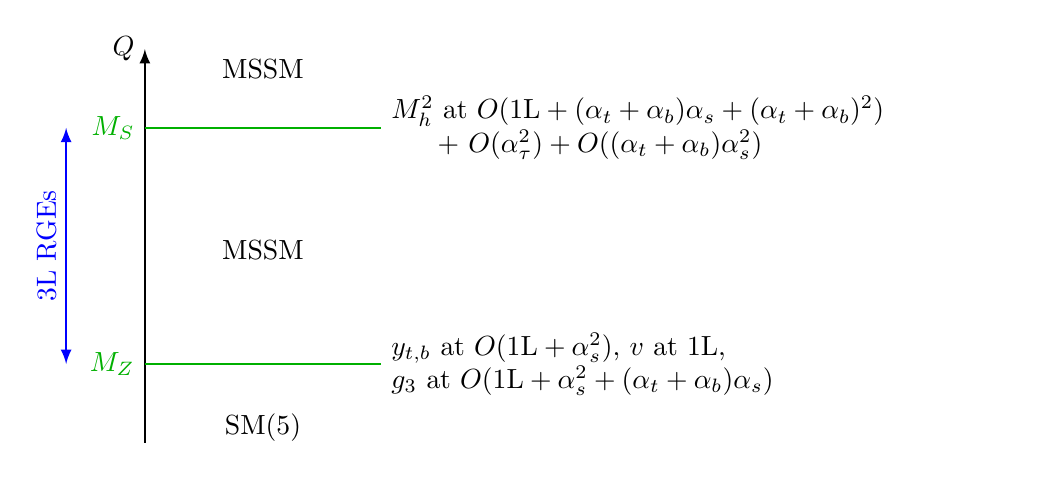
\begin{tikzpicture}
    \path[arrow] (0,0) -- (0,5) node[left]{$Q$};
    \draw[thick,darkgreen] (0,4) node[left]{$M_S$} -- node[above = 0.5cm,black]{MSSM} (3,4) node[right,black,text width=8cm]{
      $M_h^2$ at $O(\text{1L} + (\at+\ab)\as + (\at+\ab)^2)$\\ \ \ \ \ \ + $O(\atau^2) + O((\at + \ab)\as^2)$};
    \draw[thick,darkgreen] (0,1) node[left]{$M_Z$} -- node[above = 1.2cm,black]{MSSM} node[below = 0.5cm,black]{SM(5)} (3,1) node[right,black,text width=8cm]{
      $y_{t,b}$ at $O(\text{1L} + \as^2)$, $v$ at 1L, \\ $g_3$ at $O(\text{1L} + \as^2 + (\at + \ab)\as)$};
    \path[arrow,latex-latex,blue] (-1,1) -- node[above,rotate=90]{3L RGEs} (-1,4);
  \end{tikzpicture}
  \end{center}
  $M_h^2$: \mycite{0105096, 0112177, 0212132, 0206101, 0305127, 1708.05720}\\
  $y_{t,b}$: \mycite{0210258, 0507139, 0707.0650, 0912.4652},
  $g_3$: \mycite{0509048, 0810.5101, 1009.5455}\\
  $\beta_i$: \mycite{0308231, 0408128}
\end{frame}

\subsection{EFT calculation}

\begin{frame}{EFT calculation (\texttt{HSSUSY})}
  \begin{center}
    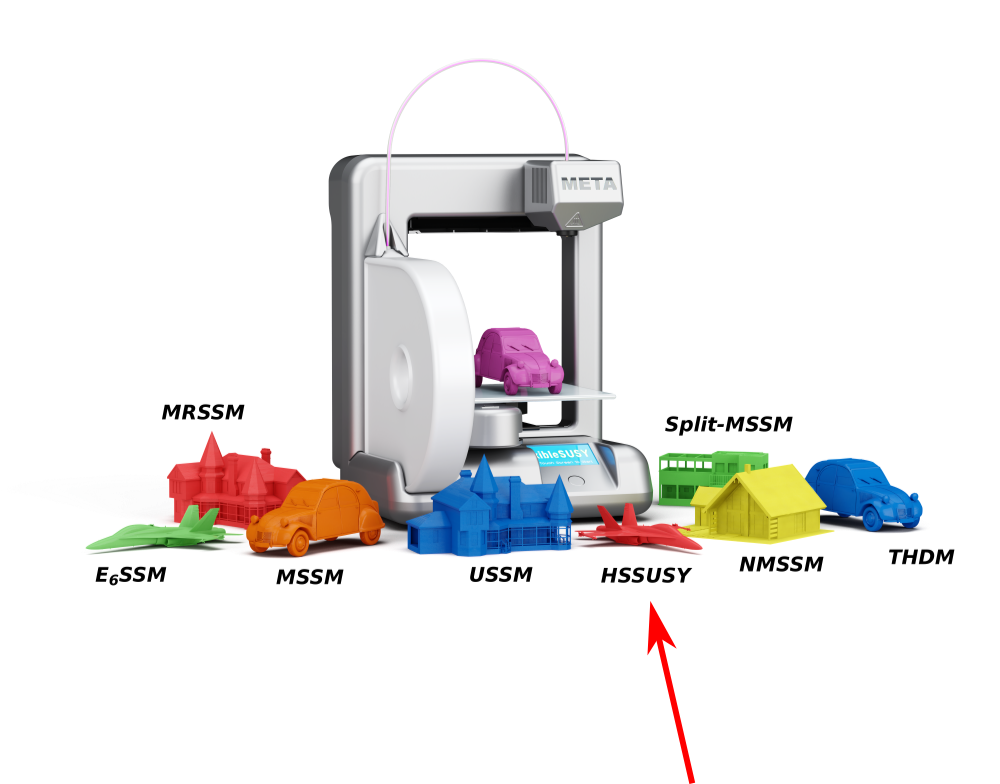
\includegraphics[width=0.8\textwidth]{images/FS-HSSUSY.png}
  \end{center}
\end{frame}

\begin{frame}{EFT calculation (\texttt{HSSUSY})}
  \begin{center}
  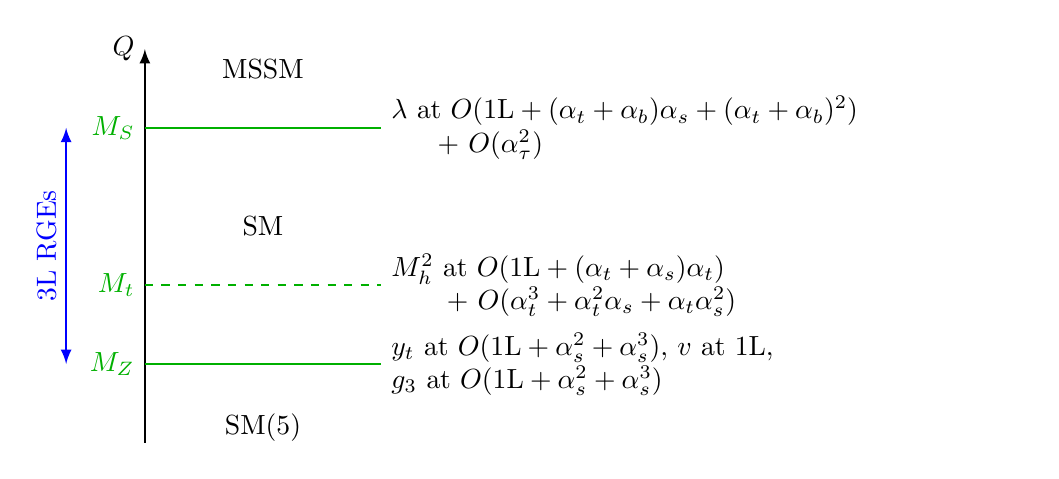
\begin{tikzpicture}
    \path[arrow] (0,0) -- (0,5) node[left]{$Q$};
    \draw[thick,darkgreen] (0,4) node[left]{$M_S$} -- node[above = 0.5cm,black]{MSSM} (3,4) node[right,black,text width=8cm]{
      $\lambda$ at $O(\text{1L} + (\at+\ab)\as + (\at+\ab)^2)$\\ \ \ \ \ \ + $O(\atau^2)$};
    \draw[thick,dashed,darkgreen] (0,2) node[left]{$M_t$} -- (3,2) node[right,black,text width=8cm]{
      $M_h^2$ at $O(\text{1L} + (\at+\as)\at)$\\ \ \ \ \ \ \ + $O(\at^3 + \at^2\as + \at\as^2)$
    };
    \draw[thick,darkgreen] (0,1) node[left]{$M_Z$} -- node[above = 1.5cm,black]{SM} node[below = 0.5cm,black]{SM(5)} (3,1) node[right,black,text width=8cm]{
      $y_t$ at $O(\text{1L} + \as^2 + \as^3)$, $v$ at 1L, \\ $g_3$ at $O(\text{1L} + \as^2 + \as^3)$};
    \path[arrow,latex-latex,blue] (-1,1) -- node[above,rotate=90]{3L RGEs} (-1,4);
  \end{tikzpicture}
  \end{center}
  $\lambda$: \mycite{1407.4081, 1504.05200, 1703.08166}
  $M_h^2$: \mycite{1205.6497, 1504.05200, 1407.4336}\\
  $y_t$: \mycite{9912391, 1205.2892},
  $g_3$: \mycite{9305305, 9707474, 9708255, 0004189}\\
  $\beta_i$: \mycite{1201.5868, 1210.6873, 1212.6829, 1205.2892, 1303.4364}
\end{frame}

\section{Uncertainty estimates}

%%%%%%%%%%%%%%%%%%%%%%%%%%%%%%%%%%%%%%%%
\begin{frame}{Contents}
  \tableofcontents[currentsection]
\end{frame}
%%%%%%%%%%%%%%%%%%%%%%%%%%%%%%%%%%%%%%%%

\subsection{Fixed-order calculation}

\begin{frame}{Fixed-order calculation}
  \begin{center}
    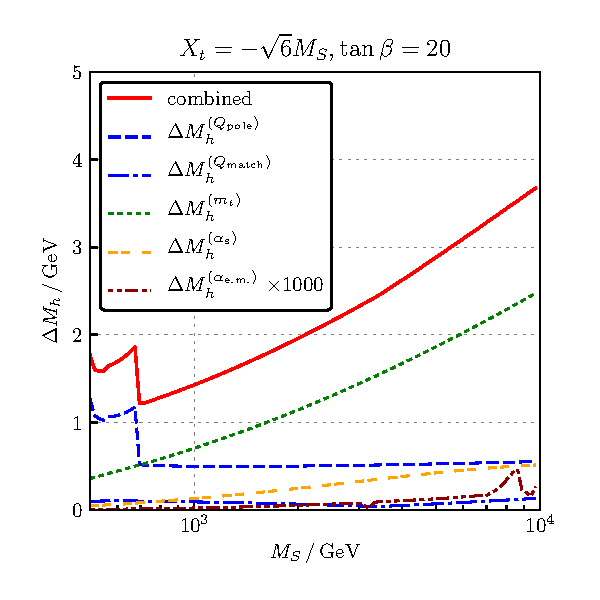
\includegraphics[width=0.49\textwidth]{plots/kuts-9/SS_TB-20_Xt--sqrt6_individual}
  \end{center}
\end{frame}

\subsection{EFT calculation}

\begin{frame}{EFT calculation}
  \begin{center}
    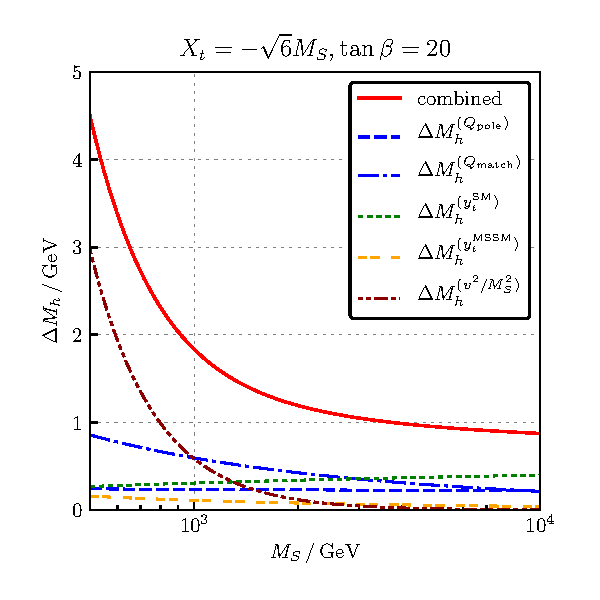
\includegraphics[width=0.49\textwidth]{plots/kuts-9/HSSUSY_TB-20_Xt--sqrt6_individual}
  \end{center}
\end{frame}

\section{When should the EFT be used?}

%%%%%%%%%%%%%%%%%%%%%%%%%%%%%%%%%%%%%%%%
\begin{frame}{Contents}
  \tableofcontents[currentsection]
\end{frame}
%%%%%%%%%%%%%%%%%%%%%%%%%%%%%%%%%%%%%%%%

\begin{frame}{When should the EFT be used?}
  \begin{center}
    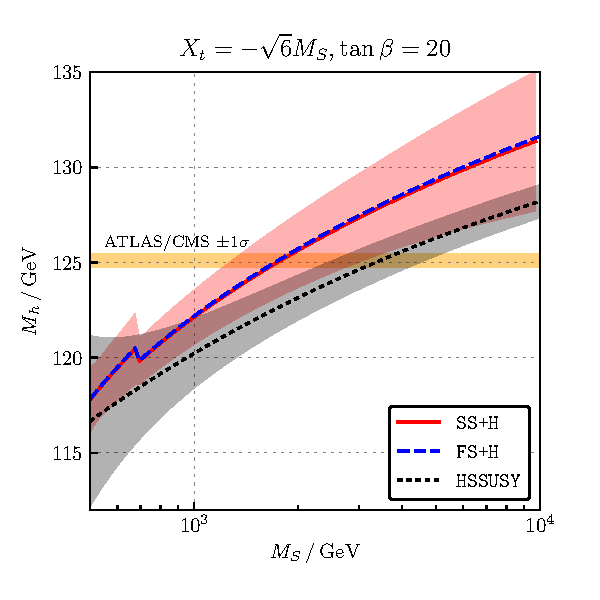
\includegraphics[width=0.49\textwidth]{plots/kuts-9/Mh_MS_TB-20_Xt--sqrt6}
  \end{center}
\end{frame}

\section{How heavy can the lightest stop be?}

%%%%%%%%%%%%%%%%%%%%%%%%%%%%%%%%%%%%%%%%
\begin{frame}{Contents}
  \tableofcontents[currentsection]
\end{frame}
%%%%%%%%%%%%%%%%%%%%%%%%%%%%%%%%%%%%%%%%

\begin{frame}{How heavy can the lightest stop be?}
  \begin{center}
    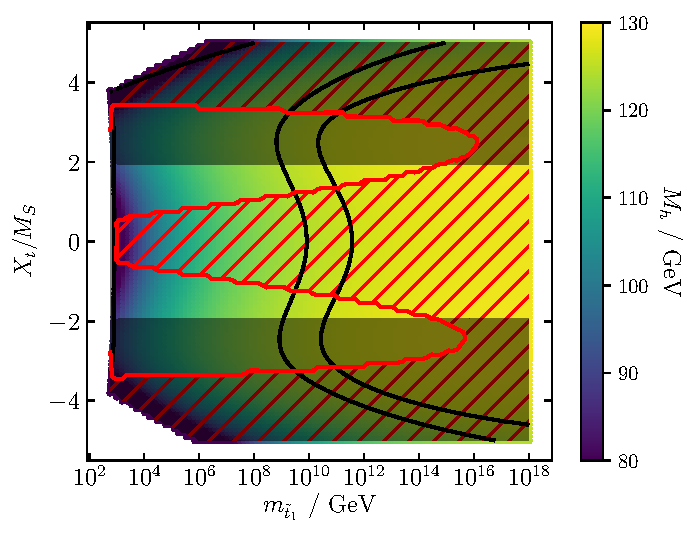
\includegraphics[width=0.49\textwidth]{{{plots/kuts-9/TB-1}}}\hfill
    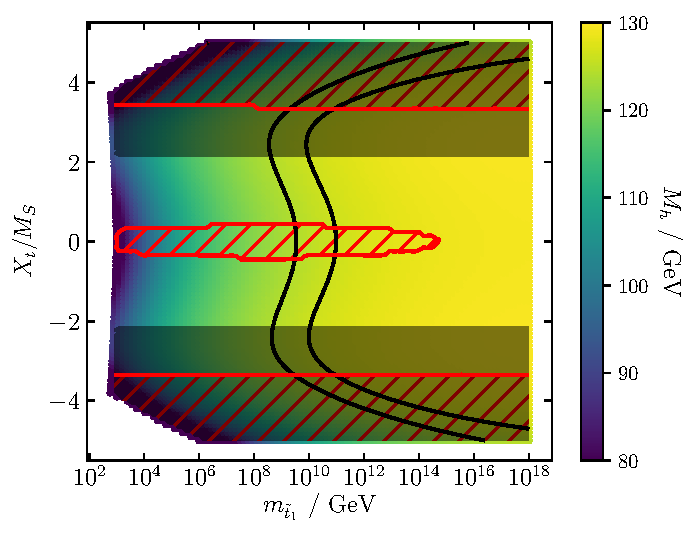
\includegraphics[width=0.49\textwidth]{{{plots/kuts-9/TB-1.2}}}
  \end{center}
\end{frame}

\begin{frame}[noframenumbering]
  \begin{center}
    \Huge Backup
  \end{center}
\end{frame}

\begin{frame}[noframenumbering]{Uncertainty estimate}
  Fixed-order calculation (\texttt{FS+H}):
  \begin{itemize}
  \item vary $Q_\pole \in [\MS/2, 2\MS]$
  \item $\alpha^{1L}_s(M_Z)$ vs.\ $\alpha^{2L}_s(M_Z)$
  \end{itemize}
  EFT calculation (\texttt{HSSUSY}):
  \begin{itemize}
  \item vary $Q_\pole \in [M_t/2, 2 M_t]$ \hfill [SM uncertainty]
  \item $y_t^{2L}(M_Z)$ vs.\ $y_t^{3L}(M_Z)$ \hfill [SM uncertainty]
  \item $\lambda(\MS)$ vs.\ $\lambda(\MS) + v^2/\MS^2$ \hfill [EFT uncertainty]
  \item vary $Q_\match \in [\MS/2, 2 \MS]$ \hfill [SUSY uncertainty]
  \item $y_t^{\SM}(\MS)$ vs.\ $y_t^{\MSSM}(\MS)$ \hfill [SUSY uncertainty]
  \end{itemize}
  Hybrid calculation (\texttt{FlexibleEFTHiggs}):
  \begin{itemize}
  \item vary $Q_\pole \in [M_t/2, 2 M_t]$ \hfill [SM uncertainty]
  \item $y_t^{2L}(M_Z)$ vs.\ $y_t^{3L}(M_Z)$ \hfill [SM uncertainty]
  \item vary $Q_\match \in [\MS/2, 2 \MS]$ \hfill [SUSY uncertainty]
  \end{itemize}
\end{frame}

\begin{frame}[noframenumbering]{Determination of $g_3(M_Z)$}
  \emph{Input:} \ \ $\alpha_{\text{s}}^{\SM(5)}(M_Z) = 0.1185$\\[1em]
  $\rightarrow$
  \begin{align*}
    \alpha_{\text{s}}(M_Z) &=
    \frac{\alpha_{\text{s}}^{\SM(5)}(M_Z)}{1
      - \Delta\alpha_{\text{s}}^{1L}(M_Z)
      - \Delta\alpha_{\text{s}}^{2L}(M_Z)
      - \Delta\alpha_{\text{s}}^{3L}(M_Z)
    }
  \end{align*}
  \\\vspace{2em}
  SM: $O(\as + \as^2 + \as^3)$ \mycite{9305305, 9707474, 9708255, 0004189}\\
  split-MSSM: $O(\as)$ \mycite{9305305, 9707474, 9708255, 0004189}\\
  MSSM: $O(\as + \as^2 + (\at + \ab)\as)$ \mycite{0509048, 0810.5101, 1009.5455}
\end{frame}

\begin{frame}[noframenumbering]{Determination of $m_t(M_Z)$}
  \emph{Input:} \ \ $M_t = 173.34\eh{GeV}$\\[1em]
  $\rightarrow$
  \begin{align*}
    m_{t}(M_Z) &= M_t +
    \re\Sigma_{t}^{S}(M_Z) \\
    &\phantom{={}} + M_t \Big[ \re\Sigma_{t}^{L}(M_Z) +
    \re\Sigma_{t}^{R}(M_Z) \\
    &\phantom{={}} \qquad\quad
      + \Delta m_t^{1L} + \Delta m_t^{2L} + \Delta m_t^{3L} \Big]
  \end{align*}
  SM: $O(\text{1L} + \as^2 + \as^3)$ \mycite{9912391, 1205.2892} \\
  split-MSSM: $O(\text{1L} + \as^2)$ \mycite{1312.5220}\\
  MSSM: $O(\text{1L} + \as^2)$ \mycite{0210258, 0507139}
\end{frame}

\begin{frame}[noframenumbering]{Determination of $m_b^{\MSSM}(M_Z)$}
  \emph{Input:} \ \ $m_b^{\SM(5),\MSbar}(m_b) = 4.18\eh{GeV}$\\[1em]
  $\rightarrow$ running to $m_b^{\SM(5),\MSbar}(M_Z)$ at $O(\aem + \as^3)$\\[1em]
  $\rightarrow$ convert to $m_b^{\SM(5),\DRbar}(M_Z)$ at $O(\aem + \as)$\\[1em]
  $\rightarrow$
  \begin{align*}
    m_b(M_Z) &= \frac{m_b^{\SM(5),\DRbar}(M_Z)}{1 - \Delta m_b^{1L} - \Delta m_b^{2L}} \,, \\
    \Delta m_b^{1L} &= \Sigma_{b}^S(p^2=(m_b^{\SM(5)})^2,M_Z)/m_b\\
           &\phantom{={}}+ \Sigma_{b}^L(p^2=(m_b^{\SM(5)})^2,M_Z)
             + \Sigma_{b}^R(p^2=(m_b^{\SM(5)})^2,M_Z)\\
    \Delta m_b^{2L} &= \Delta m_b^{2L,\text{dec}} - \frac{\as}{3\pi}\Delta m_b^{1L}
  \end{align*}
  with $\Delta m_b^{2L,\text{dec}}$ at $O(\as^2)$ from \mycite{0707.0650, 0810.5101}
\end{frame}

\begin{frame}[noframenumbering]{Determination of $v(M_Z)$}
  \emph{Input:} \ \ $M_Z = 91.1876\eh{GeV}$\\[1em]
  $\rightarrow$
  \begin{align*}
    v(M_Z) &= \frac{2 m_Z(M_Z)}{\sqrt{g_Y^2(M_Z) + g_2^2(M_Z)}} \\
    m_Z(M_Z) &= \sqrt{M_Z^2 + \Pi_Z^{1L}(p^2=M_Z^2,Q=M_Z)}
  \end{align*}
\end{frame}

\begin{frame}[noframenumbering]{Determination of $g_1$ and $g_2$ as in BPMZ \mycite{9606211}}
  \emph{Input:} \ \ $\aem^{\SM(5)}(M_Z) = 1/127.916$, $G_F = 1.1663787\cdot 10^{-5}\text{GeV}^2$\\[1em]
  $\rightarrow$
  \begin{align*}
  \aem(M_Z) &=
  \frac{\aem^{\SM(5)}(M_Z)}{1 - \Delta\aem^{1L}(M_Z)} 
  \end{align*}
  \begin{align*}
    g_1(M_Z) &= \sqrt{\frac{5}{3}} \frac{\sqrt{4\pi\aem(M_Z)}}{\cos\theta_w(M_Z)} \,, &
    g_2(M_Z) &= \frac{\sqrt{4\pi\aem(M_Z)}}{\sin\theta_w(M_Z)}
  \end{align*}
  \begin{align*}
  \sin^2\theta_w \cos^2\theta_w =
  \frac{\pi\,\aem}{\sqrt{2} M_Z^2 G_F (1-\delta_r)}
  \end{align*}
  \begin{align*}
    \delta_r &= \hat\rho \frac{\re\Sigma_{W,T}(0)}{M_W^2} -
    \frac{\re\Sigma_{Z,T}(M_Z^2)}{M_Z^2} + \delta_{\text{VB}} + \delta_r^{(2)} \\
    \hat\rho &= \frac{1}{1-\Delta\hat\rho} , \qquad \Delta\hat\rho
    = \re\Biggl[ \frac{\Sigma_{Z,T}(M_Z^2)}{\hat\rho\,M_Z^2} -
    \frac{\Sigma_{W,T}(M_W^2)}{M_W^2}\Biggr] + \Delta\hat\rho^{(2)}
  \end{align*}
\end{frame}

\begin{frame}[noframenumbering]{Determination of $M_h^2$ in the SM and split-MSSM}
  \emph{SM}:
  Iterate until $p^2 = M_h^2$:
  \begin{align*}
    M_h^2 &= m_h^2 + (\Delta m_h^2)_{1L}(p^2)
            + (\Delta m_h^2)_{2L}(p^2) +(\Delta m_h^2)_{3L}
  \end{align*}
  $O(\text{1L} + (\at+\as)\at + (\at^2 + \at\as + \as^2)\at)$\\
  \mycite{1205.6497, 1504.05200, 1407.4336}\\
  Note: $O(\at^3)$ incomplete due to missing $p^2$-dependence of $O(\at^2)$
  \\[2em]
  \emph{split-MSSM}:
  Iterate until $p^2 = M_h^2$:
  \begin{align*}
    M_h^2 &= m_h^2 + (\Delta m_h^2)_{1L}(p^2)
            + (\Delta m_h^2)_{2L} +(\Delta m_h^2)_{3L}
  \end{align*}
  split-MSSM: $O(\text{1L} + (\at+\as)\at + \at\as^2)$
  \mycite{1205.6497, 1312.5220}
\end{frame}

\begin{frame}[noframenumbering]{Determination of $M_h^2$ in the MSSM}
  Iterate until $p^2 = M_h^2$:
  \begin{align*}
    M_h^2 &= \Eigenvalue\Big[
            m_h^2 + (\Delta m_h^2)_{1L}(p^2)
            + (\Delta m_h^2)_{2L} + (\Delta m_h^2)_{3L}
            \Big]
  \end{align*}
  MSSM: $O(\text{1L} + (\at+\ab)\as + (\at+\ab)^2 + \atau^2 + (\at + \ab)\as^2)$\\
  \hspace{2em} \mycite{0105096, 0112177, 0212132, 0206101, 0305127, 1708.05720}
\end{frame}

\begin{frame}[noframenumbering]{Determination of $\lambda$ in the FlexibleEFTHiggs\\ \mycite{1609.00371, 1703.03267, 1710.03760}}
  Matching condition:
  \begin{align*}
    (M_h^2)_{\SM} &\overset{!}{=} (M_h^2)_{\MSSM} \qquad \text{at 1L at } Q = \MS
  \end{align*}
  With $(M_h^2)_{\SM} = \lambda v^2 + (\Delta m_h^2)_{\SM}$\\
  $\Rightarrow$
  \begin{align*}
    \lambda(\MS) &= \frac{1}{v^2} \left[ (M_h^2)_{\MSSM} - (\Delta m_h^2)_{\SM} \right]
  \end{align*}
\end{frame}

\end{document}
